\documentclass[notitlepage,a4paper,10pt]{article} % draft is for debug, titlepage will make a document cover
\pagestyle{plain} % "headings" or "plain"

\usepackage{textcomp} % for the ° in author
\usepackage{amsmath} % base math commands
\usepackage{xcolor}
\usepackage[pdftex]{graphicx} % for include images.
\usepackage[utf8]{inputenc} % make it understand accents.
\usepackage[english]{babel} % specify language for auto-generated texts.
\usepackage{csquotes} % for quotations
\usepackage{soul} % for erasing lines over text (using \st{text})
\usepackage{bm} % for bold vector notation on equations

% % cool fonts
% \usepackage{gfsartemisia}
\usepackage{gentium}
\usepackage[T1]{fontenc}

% \usepackage{amssymb} % for def equals \triangleq
\usepackage[pdftex,bookmarks=false]{hyperref}
\hypersetup{%
	pdfmenubar=false,%
	pdffitwindow=true,%
	colorlinks=true,%
	linkcolor=blue,%
	citecolor=blue,%
	urlcolor=blue,%
	pdftitle={Patriot - Michael Mugnai},%
	pdfauthor={Michael Mugnai}}

\frenchspacing
\graphicspath{{img/}}

\newcommand{\ud}{\,\mathrm{d}} % "d" to put at end of integrals

\title{Patriot Project \\
	\large Real Time Systems A.A. 2016/17}
\author{Michael~Mugnai\\n\textdegree 556448\\m.mugnai@ymail.com \\ \\ \\
	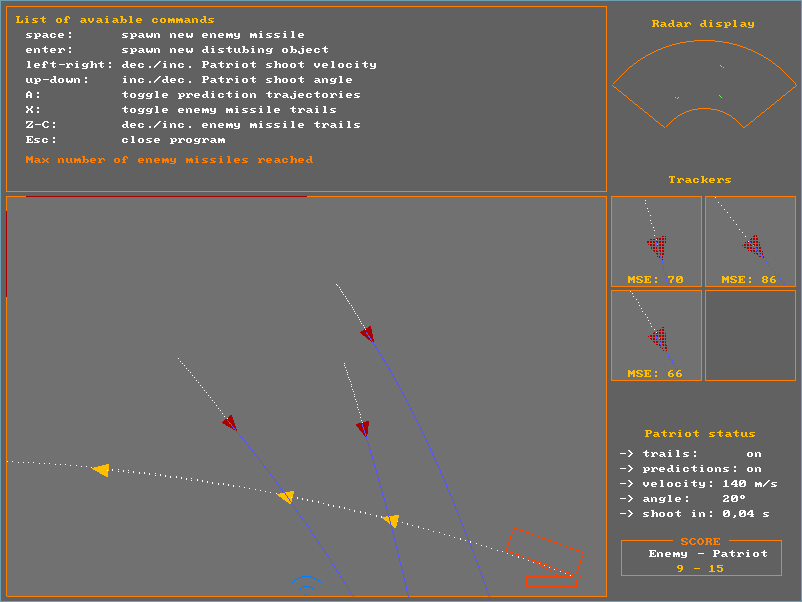
\includegraphics[width=\textwidth]{cover.png}}
\date{Delivery date: not today}

\begin{document}

\maketitle

\begin{abstract} % Quick summary of the document.
	A report must be produced (8-10 pages) to explain the project details. The delivery date.
	The report must include a general description of the project, the design choices, the user interface,
	the shared data structures, the tasks involved, a taskresource diagram, a discussion on the task
	parameters (how they were defined), and a set of experimental results. Figures and screenshots are welcome.
	Task code must not be included in the report.
\end{abstract}

\newpage
\hypersetup{linkcolor=black}
\tableofcontents
\hypersetup{linkcolor=blue}
\newpage

% \section{Assignment}
% \section{Problem definition}
% \section{Realization concepts}
% 	\subsection{Missiles}
% 		\subsubsection{Missiles characterization}
% 	\subsection{Radar}
% 	\subsection{Trackers}
% 	\subsection{Parameters evaluation}
% 		\subsubsection{Velocities}
% 		\subsubsection{Accelerations}
% 	\subsection{Rocket launcher}
% 	\subsection{Missiles interception}
% \section{Design choices}
% 	\subsection{Graphics}
% 	\subsection{Task and resources}
% \section{Results}

\section{Assignment}

	Here's what the choosen assignment said:
	\begin{displayquote}
	\emph{Simulate a set of Patriot defense missiles that identify enemy targets, predict their trajectories and are launched to catch them.}
	\end{displayquote}
	Therefore the program has to simulate a piece of sky, monitor the presence of flying objects and check if they have a ballistic tarjectory; if so, shoot them down.

\section{Problem definition}

	% ``coolApex"
	Assuming a 2-dimensional space, the ground is represented as the baseline of the so-called \emph{world box}. Let's suppose that the right side is a \emph{safe zone}: no missile can come from here. In this way, the Patriot rocket launcher can be placed on the bottom right of our world box.

	The problem can be subdivided in this parts:
	\begin{enumerate}
		\item a radar that monitors the sky and individuate every flying object;
		\item a tracking camera that follows every object pointed out by the radar;
		\item acquiring subseguent object's positions, velocities and accelerations are estimated supposing ballistic trajectories;
		\item if predicted positions correspond to real positions (within certain inaccuracy), the flying object has effectivelly a ballistic trajectory, and can be assumed as obstile;
		\item the rocket laucher evaluates estimated interception time of ostile object with launcher's trajectory (fixed), then shoot at the right time (given by Patriot time-to-fly).
	\end{enumerate}

	In this way, we can build up the program following a modular approach.

\section{Realization concepts}

	What will follow summarizes the concepts behind each element of the program.

	\subsection{Missiles}

		Missiles are central object of this program. Caracterized by ballistic motion (i.e. the only force applied is
		$m\bm{g} = \begin{bmatrix} 0 & 0 & -mg \end{bmatrix} ^T$
		), can be categorized as \emph{enemy missiles} or \emph{Patriot missiles}.

		In any case, the equations that govern missile's motion are:
		\begin{equation}
			\begin{cases}
				x = v_x t + x_0 \\
				y = - \frac{1}{2} g t^2 + v_y t + y_0
			\end{cases}
		\end{equation}
		Where a more pratical, step-increment formula can be defined:
		\begin{equation}
			\begin{cases}
				v_y^{(k+1)} = v_y^{(k)} - g \ud t_k \\
				x_{k+1} = v_x \ud t_k + x_k \\
				y_{k+1} = - \frac{1}{2} g \ud t_k^2 + v_y^{(k+1)} t + y_k
			\end{cases}
		\end{equation}
		Notice that $v_x$ is constant for the entire life of a missile.

		Current missile orientation $\alpha$ (respect to horizon) can be recovered easly:
		\begin{equation}
			\frac{v_y}{v_x} = \frac{v \sin{\alpha}}{v \cos{\alpha}} = \tan{\alpha}
			\to \alpha = \arctan{\frac{v_y}{v_x}}
		\end{equation}

		\subsubsection{Missiles characterization}

			Initial values will determinate the ``faction" of any missile:

			\begin{enumerate}

				\item \textbf{Enemy missiles}: these objects can spawn from \emph{left side} or from \emph{top} of the world box, each side with equal probability. Initial position, orientation and velocity are generated randomly in a range that guarantees a collision with the ground inside the world box;
				\item \textbf{Patriot missiles}: objects generated by the rochet launcher, thus with initial position and orientation fixed, meant to intercept enemy missiles.
			\end{enumerate}

	\subsection{Radar}

		The radar is a device located ahead of the rocket launcher, in our world box is in the mid point of the ground. From radar's origin, a beam plumbs the sky radially, until a max distance is reached.

		The purpose of the radar is to detect presence of flying objects, and communicate it to the trackers. When an object is already tracked, there's no benefit in scanning it anymore, therefore points too near to radar (thus to the ground) are useless to monitor: a minimum distance from radar's origin can be defined, and the beam starts only from there.

		The plumbed area is, since the radar is centered on our world, specular on the vertical axis: given $\theta$ the angle with the horizon, the radar aperture is $\pi - 2\theta$.

		What is seen by the radar is reproposed on top-right corner of the program.

	\subsection{Trackers}

		When the presence of something in the sky is detected, a tracking camera is responsable to enstablish what it is.

		Focusing on a square of pixels of fixed dimensions, a moving object can be observed by making the center of the view chase the barycenter of what is currently seen.

		The idea is simple: in every time-instant, pixels different from sky's color are taken into account in the evaluation of the center point; in particular, given a square image with $n$ pixels $(x_i,y_i)$ different from sky color, \emph{centroid} position is:
		\begin{equation}
			\begin{bmatrix} c_x \\ c_y \end{bmatrix} = \frac{1}{n} \sum_{i=1}^n \begin{bmatrix} x_i \\ y_i \end{bmatrix}
		\end{equation}

		Positions of subsequent time-instants are stored, allowing to estimate object's trajectory.

	\subsection{Parameters evaluation}

		Caracterizing a ballistic trajectory leads to identify two main parameters: \emph{horizontal velocity}, constant but unknown, and \emph{vertical velocity}, that increase at every time-instant with a slope of of $g$.
		% Assuming that every ostile object has a ballistic trajectory, the only force applyed to them is gravity $\bm{g}$ (vertical), therefore horizontal velocity is constant, and vertical is linear, with slope equals to $\bm{g}$.

		Since we can presume that tracker's detected positions are afflicted by error, what we're looking for is a trajectory that minimize its distance from any given point, instead of trying to evaluate an exact interpolation of them.

		\subsubsection{Horizontal velocity}

			As previously said, there's no acceleration along $x$'s axis, thus a $(x,t)$ plot will exibit a line, with inclination $v_x$.
			What we do now is to find the equation of the rect $f_{(t)} = \alpha_0 + \alpha_1 t$ that has the minimum distance with each collected point.
			This leads to look for $\alpha_0$ and $\alpha_1$ that minimize $ S_{(\alpha_0, \alpha_1)} := \sum_{i=1}^n | x_i - f_{(t_i)} |^2 $.

			\begin{equation}
				\min_{\alpha_0, \alpha_1} S_{(\alpha_0, \alpha_1)} \to
				\begin{cases}
					\frac{\partial S}{\partial \alpha_0} = -2 \sum_{i=1}^n (x_i - \alpha_0 - \alpha_1 t_i) = 0 \\
					\frac{\partial S}{\partial \alpha_1} = -2 \sum_{i=1}^n (x_i - \alpha_0 - \alpha_1 t_i) t_i = 0
				\end{cases}
			\end{equation}

			\begin{equation} \label{partder}
				\begin{cases}
					n \alpha_0 + \alpha_1 \sum_{i=1}^n t_i = \sum_{i=1}^n x_i \\
					\alpha_0 \sum_{i=1}^n t_i + \alpha_1 \sum_{i=1}^n t_i^2 = \sum_{i=1}^n x_i t_i
				\end{cases}
			\end{equation}

			\begin{equation}
					\alpha_0 = \frac
					{\sum_{i=1}^n t_i^2 \sum_{i=1}^n x_i - \sum_{i=1}^n t_i \sum_{i=1}^n x_i t_i}
					{n \sum_{i=1}^n t_i^2 - (\sum_{i=1}^n t_i)^2}
			\end{equation}

			\begin{equation} \label{xvel}
					\alpha_1 = \frac
					{n \sum_{i=1}^n t_i x_i - \sum_{i=1}^n t_i \sum_{i=1}^n x_i}
					{n \sum_{i=1}^n t_i^2 - (\sum_{i=1}^n t_i)^2}
			\end{equation}

			The purpose of all of this is to estimate $v_x$, i.e. rect's inclination $\alpha_1$, thus for us equation \eqref{xvel} is the only one relevant.

		\subsubsection{Vertical velocity}

			In a similar way we can proceed to estimate $v_y$. Since vertical acceleration is constant (equals to $-g$), the $(y,t)$ plot is parabolic, therefore $f_{(t)} = \alpha_0 + \alpha_1 t + \alpha_2 t^2$, where $\alpha_2 = -g$.

			Equation \ref{partder} changes as follows ($\frac{\partial S}{\partial \alpha_2} = 0$ is omitted because redundant):

			\begin{equation}
				\frac{\partial S}{\partial \alpha_0} = 0 \to
				n \alpha_0 + \alpha_1 \sum_{i=1}^n t_i =
					\overbrace{\sum_{i=1}^n x_i - \alpha_2 \sum_{i=1}^n t_i^2}^p
			\end{equation}
			\begin{equation}
				\frac{\partial S}{\partial \alpha_1} = 0 \to
				\alpha_0 \sum_{i=1}^n t_i + \alpha_1 \sum_{i=1}^n t_i^2 =
					\underbrace{\sum_{i=1}^n x_i t_i - \alpha_2 \sum_{i=1}^n t_i^3}_q
			\end{equation}

			\begin{equation}
					\alpha_0 = \frac
					{\sum_{i=1}^n t_i^2 p \sum_{i=1}^n x_i q}{n \sum_{i=1}^n t_i^2 - (\sum_{i=1}^n t_i)^2}
			\end{equation}

			\begin{equation} \label{yvel}
					\alpha_1 = \frac
					{n q - \sum_{i=1}^n t_i p}{n \sum_{i=1}^n t_i^2 - (\sum_{i=1}^n t_i)^2}
			\end{equation}

			As before, we're looking for $\alpha_1$, so only equation \ref{yvel} is needed.

	\subsection{Rocket launcher}

		Patriot's launcher is setted in bottom left corner of world box, giving its back to the safe zone.
		Its orientation, combined with Patriot initial velocity, determine the path that every missile launched will follow.
		\st{These parameters can be changed by user}, but it's fundamental that they produce paths that intersect enemy trajectories, otherwise there's no point of interception.

	\subsection{Missiles interception}
\section{Design choices}
	\subsection{Graphics}
	\subsection{Task and resources}
\section{Results}

% \newpage
\hypersetup{linkcolor=black}
\listoffigures % list all figures in the document, like a sort of index of images. Writes text caption contained in []
\hypersetup{linkcolor=blue}

\end{document}